\documentclass[11pt,a4paper]{article}

\usepackage[utf8]{inputenc}
\usepackage[T1]{fontenc}
\usepackage{lmodern}
\usepackage[margin=2.5cm]{geometry}
\usepackage{amsmath,amssymb}
\usepackage{graphicx}
\usepackage{booktabs}
\usepackage{xcolor}
\usepackage{listings}
\usepackage{enumitem}
\usepackage[colorlinks=true,linkcolor=blue!50!black,urlcolor=blue!50!black,citecolor=blue!50!black]{hyperref}

\definecolor{codebg}{gray}{0.95}
\lstset{
  basicstyle=\ttfamily\small,
  backgroundcolor=\color{codebg},
  frame=single, rulecolor=\color{gray!40},
  breaklines=true, columns=fullflexible,
  keepspaces=true, showstringspaces=false,
  literate={Å}{{\AA}}1 {≥}{{$\geq$}}1 {–}{{--}}1
}
\newcommand{\code}[1]{\texttt{#1}}
\newcommand{\wtb}{WanTiBEXOS}
\newcommand{\tool}{\texttt{wtb2kwant}}
\newcommand{\ket}[1]{\left|#1\right\rangle}
\newcommand{\bra}[1]{\left\langle#1\right|}

\title{\tool{} --- User Manual\\[4pt]
\large From \wtb{} tight-binding Hamiltonians to Kwant transport scripts}
\author{Version 0.1.0}
\date{\today}

\begin{document}
\maketitle

\begin{abstract}
\tool{} reads a tight-binding (TB) Hamiltonian in the \wtb{} format, together with the
Wannier-function centres from \code{wannier90.wout}, and writes a self-contained Python
script for the Kwant quantum-transport package. The generated script contains the
converted parameters and ready-to-use builders for nanoribbons and two-terminal devices,
for both band structures and transmission calculations. This manual covers installation,
usage, the input formats, the conventions and algorithms used in the conversion, the API
of the generated script, and a validation on monolayer MoS$_2$.
\end{abstract}

\tableofcontents
\newpage

%=====================================================================
\section{Overview}
%=====================================================================

The \wtb{} code reads TB Hamiltonians from two sources:
\begin{enumerate}[nosep]
  \item Wannier90 maximally localized Wannier functions. These give an orthogonal basis,
        and the file \code{tb\_hr.dat} is generated by \code{param\_gen\_vasp}.
  \item DFT codes with localized basis sets, such as SIESTA. These give a non-orthogonal
        basis with overlap matrix $S$, and the files \code{tb-*.ham} are generated by
        \code{siesta2wtb.py}.
\end{enumerate}
\tool{} turns these parameters into a Kwant model that you can use to study finite and
semi-infinite nanostructures (nanoribbons, constrictions, devices with leads) cut from the
parent crystal. The workflow is
\begin{center}
\code{tb\_hr.dat} + \code{wannier90.wout} $\;\longrightarrow\;$ \tool{} $\;\longrightarrow\;$
\code{kwant\_model.py} $\;\longrightarrow\;$ bands, $T(E)$, \dots
\end{center}

\paragraph{Design choices.}
\begin{itemize}[nosep]
  \item The output is a plain Python script, not a binary data file. It embeds all
        parameters, depends only on \code{numpy}, \code{kwant} and \code{matplotlib}, and is
        meant to be read, copied and edited.
  \item Kwant sites are \emph{atoms}. The Wannier functions (WFs) centred on an atom become
        the orbitals of that site (\code{norbs} $>1$), so a real-space cut produces a
        physically meaningful edge.
  \item Every step is validated against the original Wannier90 band structure
        (Section~\ref{sec:validation}).
\end{itemize}

\paragraph{Status (v0.1.0).}
Supported: the Wannier90-type input, 2D crystals, nanoribbons, two-terminal transmission.
SP and SOC inputs are implemented but not yet validated. Planned: the non-orthogonal
(SIESTA) format, nanotubes, and 3D crystals (Section~\ref{sec:roadmap}).

%=====================================================================
\section{Installation}
%=====================================================================

\subsection{Requirements}
\begin{itemize}[nosep]
  \item Python $\geq 3.9$, \code{numpy}, \code{kwant} ($\geq 1.4$; tested with 1.5.0),
        \code{matplotlib}.
  \item \code{conda} (Anaconda, Miniconda or Miniforge) for the automatic installer.
  \item Optional: \code{pytest}, to run the tests.
\end{itemize}

\subsection{Automatic installation (recommended)}
The script \code{install.sh} installs \tool{} into a conda environment named \code{kwant}.
If that environment does not exist, it creates it from conda-forge with \code{python},
\code{kwant}, \code{numpy} and \code{matplotlib}:
\begin{lstlisting}[language=bash]
git clone https://github.com/ac-dias/wtb2kwant.git
cd wtb2kwant
./install.sh
conda activate kwant
\end{lstlisting}
Options:
\begin{center}
\begin{tabular}{ll}
\toprule
\code{--env NAME}     & use or create another environment (default \code{kwant}) \\
\code{--no-editable}  & regular install instead of an editable one (\code{pip install -e}) \\
\code{--dev}          & also install \code{pytest} \\
\code{--python X.Y}   & Python version for a new environment (default 3.12) \\
\code{--help}         & show the help \\
\bottomrule
\end{tabular}
\end{center}
If the environment exists but Kwant or matplotlib is missing, the installer adds them.

The installer also writes two launchers into \code{bin/}. They call the environment's
Python by absolute path, so you can use them without activating conda:
\begin{lstlisting}[language=bash]
export PATH="/path/to/wtb2kwant/bin:$PATH"     # e.g. in ~/.bashrc
wtb2kwant tb_hr.dat --wout wannier90.wout -o kwant_model.py
wtb2kwant-python kwant_model.py --help         # the env's Python
\end{lstlisting}
The launchers are machine-specific and are not versioned: \code{bin/} contains only a
\code{.gitignore}. Rerun \code{install.sh} after moving the repository or the environment.
At the end, the installer checks that \code{import kwant, wtb2kwant} works and that both
the command \code{wtb2kwant} and the launchers run.

\subsection{Manual installation}
\begin{lstlisting}[language=bash]
conda create -n kwant -c conda-forge python=3.12 kwant numpy matplotlib
conda activate kwant
pip install -e .          # from the repository root
\end{lstlisting}
This installs the Python package \code{wtb2kwant} and the console command
\code{wtb2kwant}. Without installing, you can also run it as
\code{python -m wtb2kwant.cli} from the repository root.

%=====================================================================
\section{Quick start}
%=====================================================================

In the folder of a Wannier90 + \wtb{} calculation:
\begin{lstlisting}[language=bash]
# 1) convert
wtb2kwant tb_hr.dat --wout wannier90.wout -o kwant_model.py

# 2) run the built-in example: bands + transmission of zigzag and
#    armchair nanoribbons -> bands_ribbons.png, bands_ribbons_transmission.dat
python kwant_model.py
python kwant_model.py --no-transport          # bands only (fast)
python kwant_model.py --help
\end{lstlisting}
For spin-polarized calculations, give the two \code{.wout} files, spin up first:
\begin{lstlisting}[language=bash]
wtb2kwant tb_hr.dat --wout wannier90.up.wout wannier90.dn.wout
\end{lstlisting}
To use the script as a module:
\begin{lstlisting}[language=Python]
from kwant_model import make_ribbon, ribbon_bands, make_two_terminal, conductance

rib = make_ribbon("zigzag", width=25.0)            # infinite ribbon
k, E = ribbon_bands(rib)                           # E relative to E_F

syst = make_two_terminal("armchair", width=20.0, length=40.0)
# ... add disorder, potentials, vacancies to `syst` here ...
T = conductance(syst.finalized(), [-0.5, 0.0, 0.5])  # e^2/h, parallel
\end{lstlisting}

%=====================================================================
\section{Input files}
%=====================================================================

\subsection{\wtb{} Wannier-type Hamiltonian (\code{tb\_hr.dat})}
This file is produced by \code{param\_gen\_vasp}. It is a short header followed by the
full \code{wannier90\_hr.dat}:
\begin{lstlisting}
NP                         ! NP | SP | SOC
0.5   !scissors operator   ! eV
-0.9676                    ! Fermi energy (eV), from OUTCAR
  3.1655459  0.0000000  0.0000000     ! a1 (Angstrom), from unit_cell_cart
 -1.5827730  2.7414432  0.0000000     ! a2
  0.0000000  0.0000000 16.0000000     ! a3
 written on 24Apr2026 at 09:20:43     ! --- wannier90_hr.dat starts here
 11                                   ! num_wann
 147                                  ! nrpts
 1 1 1 1 1 2 1 ...                    ! degeneracies, 15 per line
 R1 R2 R3  m  n  Re(H)  Im(H)         ! nrpts * num_wann^2 lines
\end{lstlisting}
For spin-polarized (SP) calculations, the file contains two \code{hr} blocks, one after
the other: spin up, then spin down. The matrix elements are
$H_{mn}(\mathbf{R})=\bra{m,\mathbf{0}}\hat H\ket{n,\mathbf{R}}$ in eV, with $\mathbf{R}$
given as integer lattice indices. \tool{} divides each element by the degeneracy of its
$\mathbf{R}$ vector, as Wannier90 does.

\subsection{Wannier90 output (\code{wannier90.wout})}
The \code{hr} file does \emph{not} contain the positions of the orbitals, but Kwant needs
them to cut nanostructures. \tool{} takes them from \code{wannier90.wout}, which every
Wannier90 run writes:
\begin{itemize}[nosep]
  \item lattice vectors (block \code{Lattice Vectors (Ang)});
  \item atoms (block \code{Site  Fractional Coordinate  Cartesian Coordinate});
  \item the final WF centres (block \code{Final State}, lines
        \code{WF centre and spread}). If there are several such blocks (for example after a
        restart), the last one is used.
\end{itemize}
Spin-polarized runs have one \code{.wout} per spin channel, and the centres of the two
channels can differ. Both files are required and are handled independently.

\paragraph{Alternative: \code{wannier90\_centres.xyz}.}
Adding \code{write\_xyz = true} to the \code{.win} file and rerunning \code{wannier90.x}
(it reuses \code{.amn}, \code{.mmn} and \code{.eig}, so no new DFT run is needed) produces
\code{wannier90\_centres.xyz} with the same information. \tool{} does not need this file.
If you enable \code{translate\_home\_cell}, remember that the centres it writes are shifted
but the \code{hr} file is \emph{not}. Section~\ref{sec:folding} explains why this matters.

\subsection{Non-orthogonal format (planned)}
The \code{siesta2wtb.py} interface writes \code{tb-\{NP,SP,SOC\}.ham}. Each line has
Cartesian supercell offsets (in \AA), orbital indices, $\mathrm{Re}\,H$, $\mathrm{Im}\,H$
and $S$. The file comes with \code{basis\_set-*.basis}, which contains the orbital
positions. Support for this format is planned (Section~\ref{sec:roadmap}).

%=====================================================================
\section{Command-line reference}
%=====================================================================

\begin{lstlisting}
wtb2kwant INPUT --wout WOUT [WOUT] [--sites {atoms,centres}]
          [--cutoff X] [--efermi X] [-o OUTPUT]
\end{lstlisting}
\begin{center}
\begin{tabular}{p{3.6cm}p{2.2cm}p{8.2cm}}
\toprule
Option & Default & Description \\
\midrule
\code{INPUT} & --- & \wtb{} Hamiltonian (\code{tb\_hr.dat}). \\
\code{--wout F [F]} & required & \code{wannier90.wout}; for SP give two files, up then down. \\
\code{--sites} & \code{atoms} & \code{atoms}: group WFs on the nearest atom (one Kwant site
  per atom). \code{centres}: one site per WF, at its centre. Use \code{centres} for
  bond-centred WFs (e.g.\ $sp^3$ hybrids). \\
\code{--cutoff X} & $10^{-5}$ & Drop matrix elements with $|H|<X$ (eV). \\
\code{--efermi X} & from file & Override the Fermi energy (eV). \\
\code{-o FILE} & \code{kwant\_model.py} & Name of the generated script. \\
\bottomrule
\end{tabular}
\end{center}
The command prints the sites, the number of orbitals per site, the periodic directions it
detected, how many matrix elements the cutoff kept, and how many WFs had to be folded.
\tool{} warns if a WF centre is more than 1\,\AA{} from the nearest atom.

%=====================================================================
\section{Conventions and algorithms}
%=====================================================================

\subsection{Matrix-element convention}
Inside \tool{} and in the generated script,
\begin{equation}
  H_{ij}(\mathbf{R}) = \bra{i,\mathbf{0}}\hat H\ket{j,\mathbf{R}}, \qquad
  H(\mathbf{k}) = \sum_{\mathbf{R}} H(\mathbf{R})\, e^{2\pi i\,\mathbf{k}\cdot\mathbf{R}},
\end{equation}
where $\mathbf{R}$ is an integer vector in units of the lattice vectors and $\mathbf{k}$
is in fractional reciprocal coordinates. This is the Wannier90 convention. Energies are in
eV and lengths in \AA.

\subsection{Folding of Wannier centres}\label{sec:folding}
Wannier90 does not keep WF centres inside the home cell. In the MoS$_2$ test, all
11 centres lie in neighbouring cells: the Mo-$d$ WFs sit at $\mathbf{r}_\text{Mo}-\mathbf{a}_2$
and the S-$p$ WFs at $\mathbf{r}_\text{S}-\mathbf{a}_1$. Because the \code{hr} matrix
elements refer to the WFs \emph{where they actually are}, you cannot move a centre without
also changing the $\mathbf{R}$ labels of its hoppings.

Let WF $w$ have centre $\mathbf{c}_w$, and assign it to a site with home-cell position
$\mathbf{p}_s$ such that $\mathbf{c}_w \simeq \mathbf{p}_s + \mathbf{n}_w\cdot A$, with
$\mathbf{n}_w$ an integer vector. The site is the nearest atom over all periodic images,
or, with \code{--sites centres}, the centre itself. The old orbital $(w,\mathbf{R})$ is the
new orbital $(w,\mathbf{R}+\mathbf{n}_w)$, hence
\begin{equation}
  H^\text{new}_{ij}\big(\mathbf{R}+\mathbf{n}_j-\mathbf{n}_i\big) = H^\text{old}_{ij}(\mathbf{R}).
\end{equation}
This is a diagonal gauge transformation of $H(\mathbf{k})$, so the eigenvalues are
unchanged. It is nevertheless essential for Kwant: without it, a ribbon edge would cut
through the wrong bonds.

\subsection{Post-processing}
\begin{itemize}[nosep]
  \item \textbf{Hermitization:} $H(\mathbf{R}) \leftarrow \tfrac12\big[H(\mathbf{R}) + H(-\mathbf{R})^\dagger\big]$.
  \item \textbf{Cutoff:} elements with $|H|<$ \code{cutoff} are set to zero, and empty
        $\mathbf{R}$ blocks are removed. Imaginary parts below $10^{-5}$\,eV are omitted
        from the script.
  \item \textbf{Periodic directions:} direction $d$ counts as periodic if some element with
        $R_d\neq 0$ survives the cutoff. For a slab with vacuum this gives two directions.
  \item \textbf{Energy reference:} with \code{SHIFT\_TO\_FERMI = True} (the default in
        the script), $E_F$ is subtracted from the on-site blocks, so all energies are
        relative to the DFT Fermi level of the bulk crystal.
  \item \textbf{Scissors operator:} it is recorded in the script (\code{SCISSORS}) but
        \emph{not} applied.
\end{itemize}

\subsection{Kwant representation}
A \code{kwant.lattice.general} is built with one sublattice per site and
\code{norbs} equal to the number of WFs on it. The bulk template has the full 2D
translational symmetry. Kwant's convention is \code{syst[a, b]} $=\bra{a}\hat H\ket{b}$,
and \code{HoppingKind(d, a, b)} denotes the pairs $(a(\mathbf{x}+\mathbf{d}), b(\mathbf{x}))$.
Therefore
\begin{equation}
  \texttt{bulk[HoppingKind}(-\mathbf{R},\, s,\, t)\texttt{]} = \bra{s,\mathbf{0}}\hat H\ket{t,\mathbf{R}}.
\end{equation}
The script stores only one block of each Hermitian pair $\{(\mathbf{R},s,t),(-\mathbf{R},t,s)\}$.
Kwant generates the conjugate block.

\subsection{Long-range hoppings, ribbon bands and lead supercells}
Wannier hoppings decay slowly. In MoS$_2$, elements above $10^{-5}$\,eV reach 7 lattice
constants. Kwant's \code{InfiniteSystem} (used for leads and for \code{kwant.physics.Bands})
only accepts hoppings between \emph{neighbouring} unit cells. \tool{} deals with this in
two ways:
\begin{enumerate}[nosep]
  \item \textbf{Ribbon bands} are computed by \code{ribbon\_hk}. It builds the Bloch
        Hamiltonian $H(k)=\sum_n h_n e^{ikn}$ directly from the hoppings of a Kwant builder
        with the \emph{primitive} ribbon period, using \code{symmetry.which} and
        \code{symmetry.to\_fd}, without finalizing it. The bands are therefore exact and
        not folded.
  \item \textbf{Leads} use a supercell of $N$ primitive periods. \code{min\_supercell}
        starts from a geometric estimate and increases $N$ until Kwant can finalize the
        ribbon. A purely geometric choice is not enough, because Kwant's fundamental domain
        is defined in tag space and is oblique in real space. For 20\,\AA{} MoS$_2$
        ribbons, $N=9$ (zigzag) and $N=4$ (armchair).
\end{enumerate}
The scattering region must be at least one lead cell long. \code{make\_two\_terminal}
lengthens it automatically if needed.

%=====================================================================
\section{The generated script}
%=====================================================================

\subsection{Structure}
\begin{enumerate}[nosep]
  \item A header comment with run instructions, and a docstring with the input files,
        sites, conversion notes and conventions.
  \item \textbf{Parameters:} \code{SYSTYPE}, \code{EFERMI}, \code{SCISSORS},
        \code{SHIFT\_TO\_FERMI}, \code{PRIM\_VECS} (\AA), \code{SITES} (name, species,
        position, orbital labels), \code{ONSITE} (one block per site) and
        \code{HOPPINGS} (list of \code{(R, s, t, block)} with
        $\text{block}=\bra{s,\mathbf{0}}\hat H\ket{t,\mathbf{R}}$).
  \item \textbf{Builders and tools} (Table~\ref{tab:api}).
  \item \code{main()}: the zigzag/armchair example, with bands, top views and transmission.
\end{enumerate}

\begin{table}[h]
\centering
\caption{Functions available in the generated script. Energies are relative to $E_F$
when \code{SHIFT\_TO\_FERMI = True}.}
\label{tab:api}
\begin{tabular}{p{5.6cm}p{9cm}}
\toprule
Function & Description \\
\midrule
\code{make\_lattice()} & Kwant polyatomic lattice (one sublattice per site). \\
\code{make\_bulk(lat=None)} & Bulk builder with 2D symmetry (template for \code{fill}). \\
\code{bulk\_hk(kfrac)} & Bulk $H(\mathbf{k})$, $\mathbf{k}$ fractional (NumPy only). \\
\code{ribbon\_period(kind)} & Period vector for \code{"zigzag"} ($\mathbf{a}_1$),
  \code{"armchair"} (shortest integer vector $\perp\mathbf{a}_1$) or any \code{(m, n)}. \\
\code{make\_ribbon(kind, width, supercell=1)} & Infinite ribbon of width \code{width} (\AA). \\
\code{ribbon\_hk(rib)}, \code{ribbon\_bands(rib, nk)} & Exact ribbon $H(k)$ and bands for any
  hopping range. \\
\code{min\_supercell(kind, width)} & Smallest lead supercell that Kwant can finalize. \\
\code{make\_two\_terminal(kind, width, length)} & Scattering region and two ribbon leads. \\
\code{conductance(syst, energies, nproc)} & $T_{0\to1}(E)$ in $e^2/h$ (no spin factor),
  parallelized over energies. \\
\code{channel\_count(rib, energies)} & Number of right-moving bands: the expected $T$ of a
  perfect ribbon. \\
\code{ribbon\_info}, \code{plot\_ribbon\_top} & Sites per cell; top view of the ribbon. \\
\code{landauer\_current(E, T, V, kT)} & Landauer current $I(V)$ in $\mu$A from a tabulated $T(E)$. \\
\code{run\_iv(widths, vmax, ...)} & Fine $T(E)$ and $I$--$V$ curves of both ribbons, with figure and data files. \\
\bottomrule
\end{tabular}
\end{table}

\subsection{Command-line options of the example}
\begin{lstlisting}
python kwant_model.py [--width-zz W] [--width-ac W] [--emin E] [--emax E]
                      [--nk NK] [--no-transport] [--ne NE] [--length L]
                      [--nproc P] [--hop-cutoff X] [-o FIGURE]
python kwant_model.py --iv [--vmax V] [--nv NV] [--de DE] [--temperature K]
                      [--hop-cutoff X] [--length L] [--nproc P] [-o FIGURE]
\end{lstlisting}
Widths and lengths are in \AA{} (default 20 and 30). The energy window defaults to
$[-3, 3]$\,eV around $E_F$, sampled with \code{--ne} 61 energies for $T(E)$. The output
is the figure (default \code{bands\_ribbons.png}) and, when transport is enabled,
\code{<figure>\_transmission.dat} with the columns $E$, $T_\text{zigzag}$ and
$T_\text{armchair}$.

With \code{--iv}, the script skips the band plots. It computes $T(E)$ on a fine grid
(step \code{--de}, default 0.01\,eV) and the $I$--$V$ curves from 0 to \code{--vmax}
(default 3\,V) at \code{--temperature} (default 300\,K), using the method of
Section~\ref{sec:iv}. If \code{--hop-cutoff} is not given, it uses $10^{-3}$\,eV. The
outputs are \code{iv\_ribbons.png}, \code{iv\_ribbons\_T.dat} and \code{iv\_ribbons\_IV.dat}.

\subsection{Ribbon geometry}
The ribbon is the strip $0 \le (\mathbf{r}-\mathbf{r}_0)\cdot\hat{\mathbf{n}} < W$, where
$\hat{\mathbf{n}}$ is the in-plane direction perpendicular to the period and $\mathbf{r}_0$
is chosen so that the home cell is included. The strip is filled from the bulk template
with \code{Builder.fill}, so the edge termination follows from where the strip boundaries
fall. Check it in the top-view panels. To get a specific termination, or to passivate or
remove dangling atoms, edit the \code{shape} functions or post-process the builder.

\subsection{Performance notes}
The cost of a transmission point is dominated by the lead-mode computation. That cost
grows with the lead cell, i.e.\ with $N\times$ the number of orbitals per ribbon period.
For the 20\,\AA{} MoS$_2$ ribbons, one energy takes about 7--8\,s on one core.
\begin{itemize}[nosep]
  \item \code{conductance} distributes the energies over processes using
        \code{multiprocessing} with \code{fork}.
  \item The calculation is memory-bound. On a 12-core/24-thread workstation, throughput
        peaks at about one process per \emph{physical} core, which is why the default is
        half the number of logical CPUs. With 12 processes, the default 61-energy example
        takes about 4 minutes per ribbon.
  \item The script sets \code{OMP\_NUM\_THREADS=1} (unless already defined) to avoid
        oversubscribing BLAS threads.
  \item For quick exploration, \code{--hop-cutoff X} (or \code{HOP\_CUTOFF} in the
        script) drops hoppings with $|H|<X$. This shrinks the lead supercell. With
        $X=10^{-3}$\,eV, the zigzag lead goes from $N=9$ to $N=5$ and each point becomes
        about 4 times faster, but the band structure changes by up to about 30\,meV and
        channel counts can change deep in the valence band. Use the full model for
        production results.
  \item \code{--no-transport} computes only the bands, which takes seconds.
\end{itemize}

%=====================================================================
\section{Validation: monolayer MoS$_2$}\label{sec:validation}
%=====================================================================

The test case is a VASP + Wannier90 calculation of monolayer MoS$_2$ without spin
polarization: 11 WFs (Mo-$d$, S-$p$), $a=3.1655$\,\AA, 16\,\AA{} of vacuum and
$E_F=-0.9676$\,eV. Running \code{tests/validate\_mos2\_np.py} reproduces every number below
and writes \code{tests/results/mos2\_np/REPORT.md}.

\subsection{Folding}
All 11 WFs had centres outside the home cell. The Mo WFs were shifted by $\mathbf{n}=(0,-1,0)$
and the S WFs by $(-1,0,0)$. The distance from each centre to its atom is between
0.006 and 0.12\,\AA. The vacuum direction was correctly identified as non-periodic.

\subsection{Bulk bands}
\begin{table}[h]
\centering
\caption{Maximum deviation from \code{wannier90\_band.dat} along $\Gamma$--K--K$'$--$\Gamma$ (301 $k$-points).}
\begin{tabular}{cccc}
\toprule
cutoff (eV) & elements kept & $\mathbf{R}$ vectors & max.\ error (meV) \\
\midrule
0         & 15431 / 15431 & 197 & 0.022 \\
$10^{-5}$ & 13621 / 15431 & 197 & 0.130 \\
$3\times10^{-5}$ & 11053 / 15431 & 195 & 0.80 \\
$10^{-4}$ & 7619 / 15431 & 153 & 3.75 \\
$10^{-3}$ & 3293 / 15431 & 63 & 31.0 \\
\bottomrule
\end{tabular}
\end{table}
The residual 0.022\,meV comes from the 6-decimal precision of the \code{hr} file.
Figure~\ref{fig:bulk} compares the bands of the generated script with the Wannier90
reference.

\begin{figure}[h]
\centering
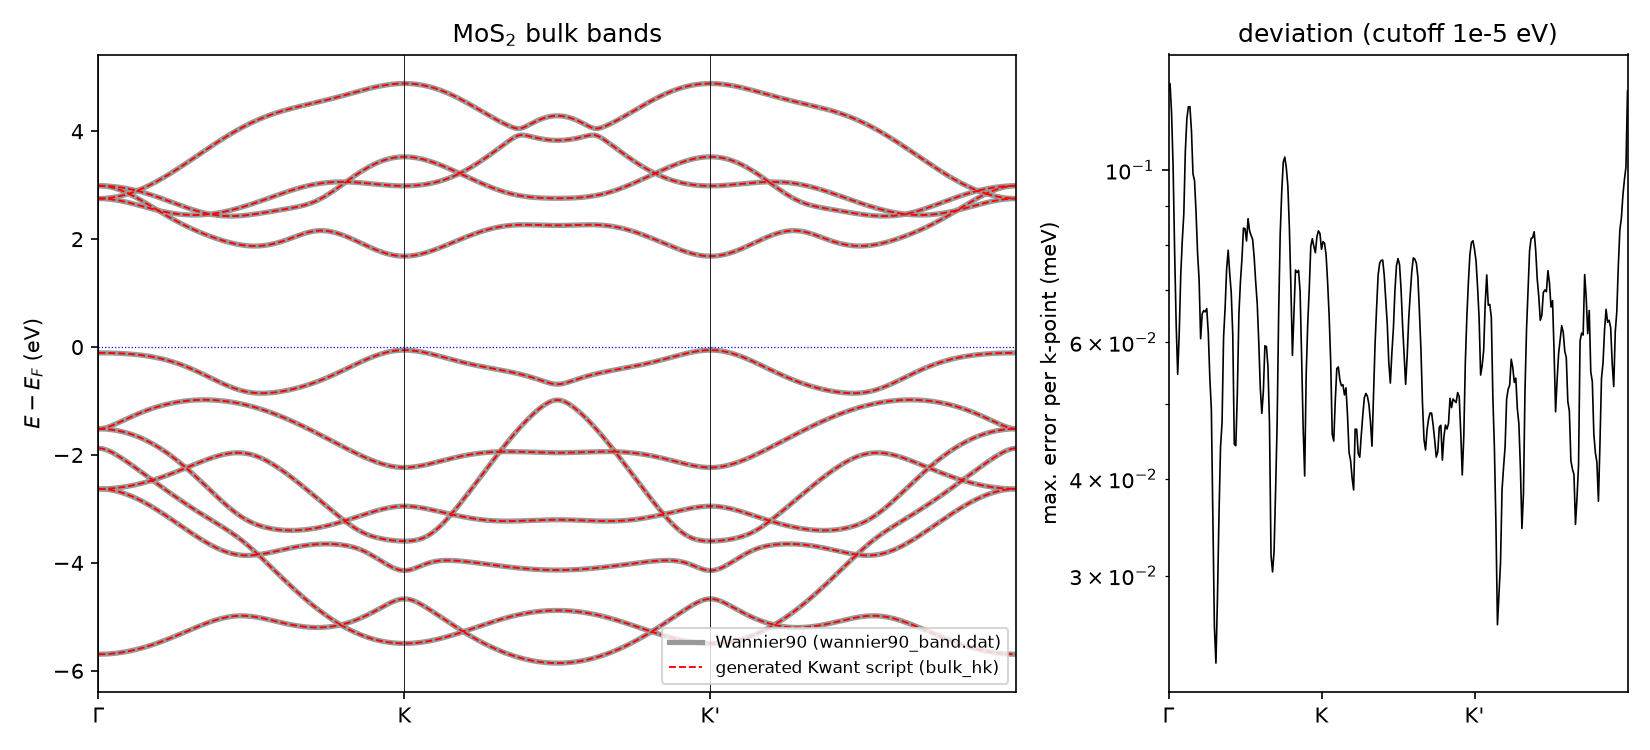
\includegraphics[width=\linewidth]{figures/bulk_bands_vs_w90.png}
\caption{Left: bulk MoS$_2$ bands from Wannier90 (grey) and from \code{bulk\_hk} of the
generated script (red dashed). Right: maximum deviation at each $k$-point (default cutoff).}
\label{fig:bulk}
\end{figure}

\subsection{Kwant conventions}
\begin{itemize}[nosep]
  \item In a finite flake of radius 40\,\AA{} built from the bulk template, all 660 hopping
        blocks satisfy \code{syst[s(0), t(R)]} $=\bra{s,\mathbf{0}}\hat H\ket{t,\mathbf{R}}$.
  \item The bands of \code{kwant.wraparound} applied to the bulk builder agree with
        \code{bulk\_hk} to $10^{-14}$\,eV.
  \item The ribbon bands from \code{ribbon\_hk} (primitive period), unfolded onto the
        supercell, agree with \code{kwant.physics.Bands} on the $N$-period supercell to
        $3\times10^{-14}$\,eV for both orientations.
\end{itemize}

\subsection{Nanoribbons and transmission}
Figure~\ref{fig:ribbons} shows 20\,\AA-wide zigzag (period $a$, 23 atoms per cell) and
armchair (period $\sqrt3 a$, 38 atoms per cell) ribbons. The zigzag ribbon is metallic,
with edge bands crossing $E_F$, as known for MoS$_2$ zigzag ribbons. The armchair ribbon
has edge states inside the bulk gap. For perfect ribbons the Kwant transmission is an
integer and equals the number of right-moving bands at every energy computed.

\begin{figure}[h]
\centering
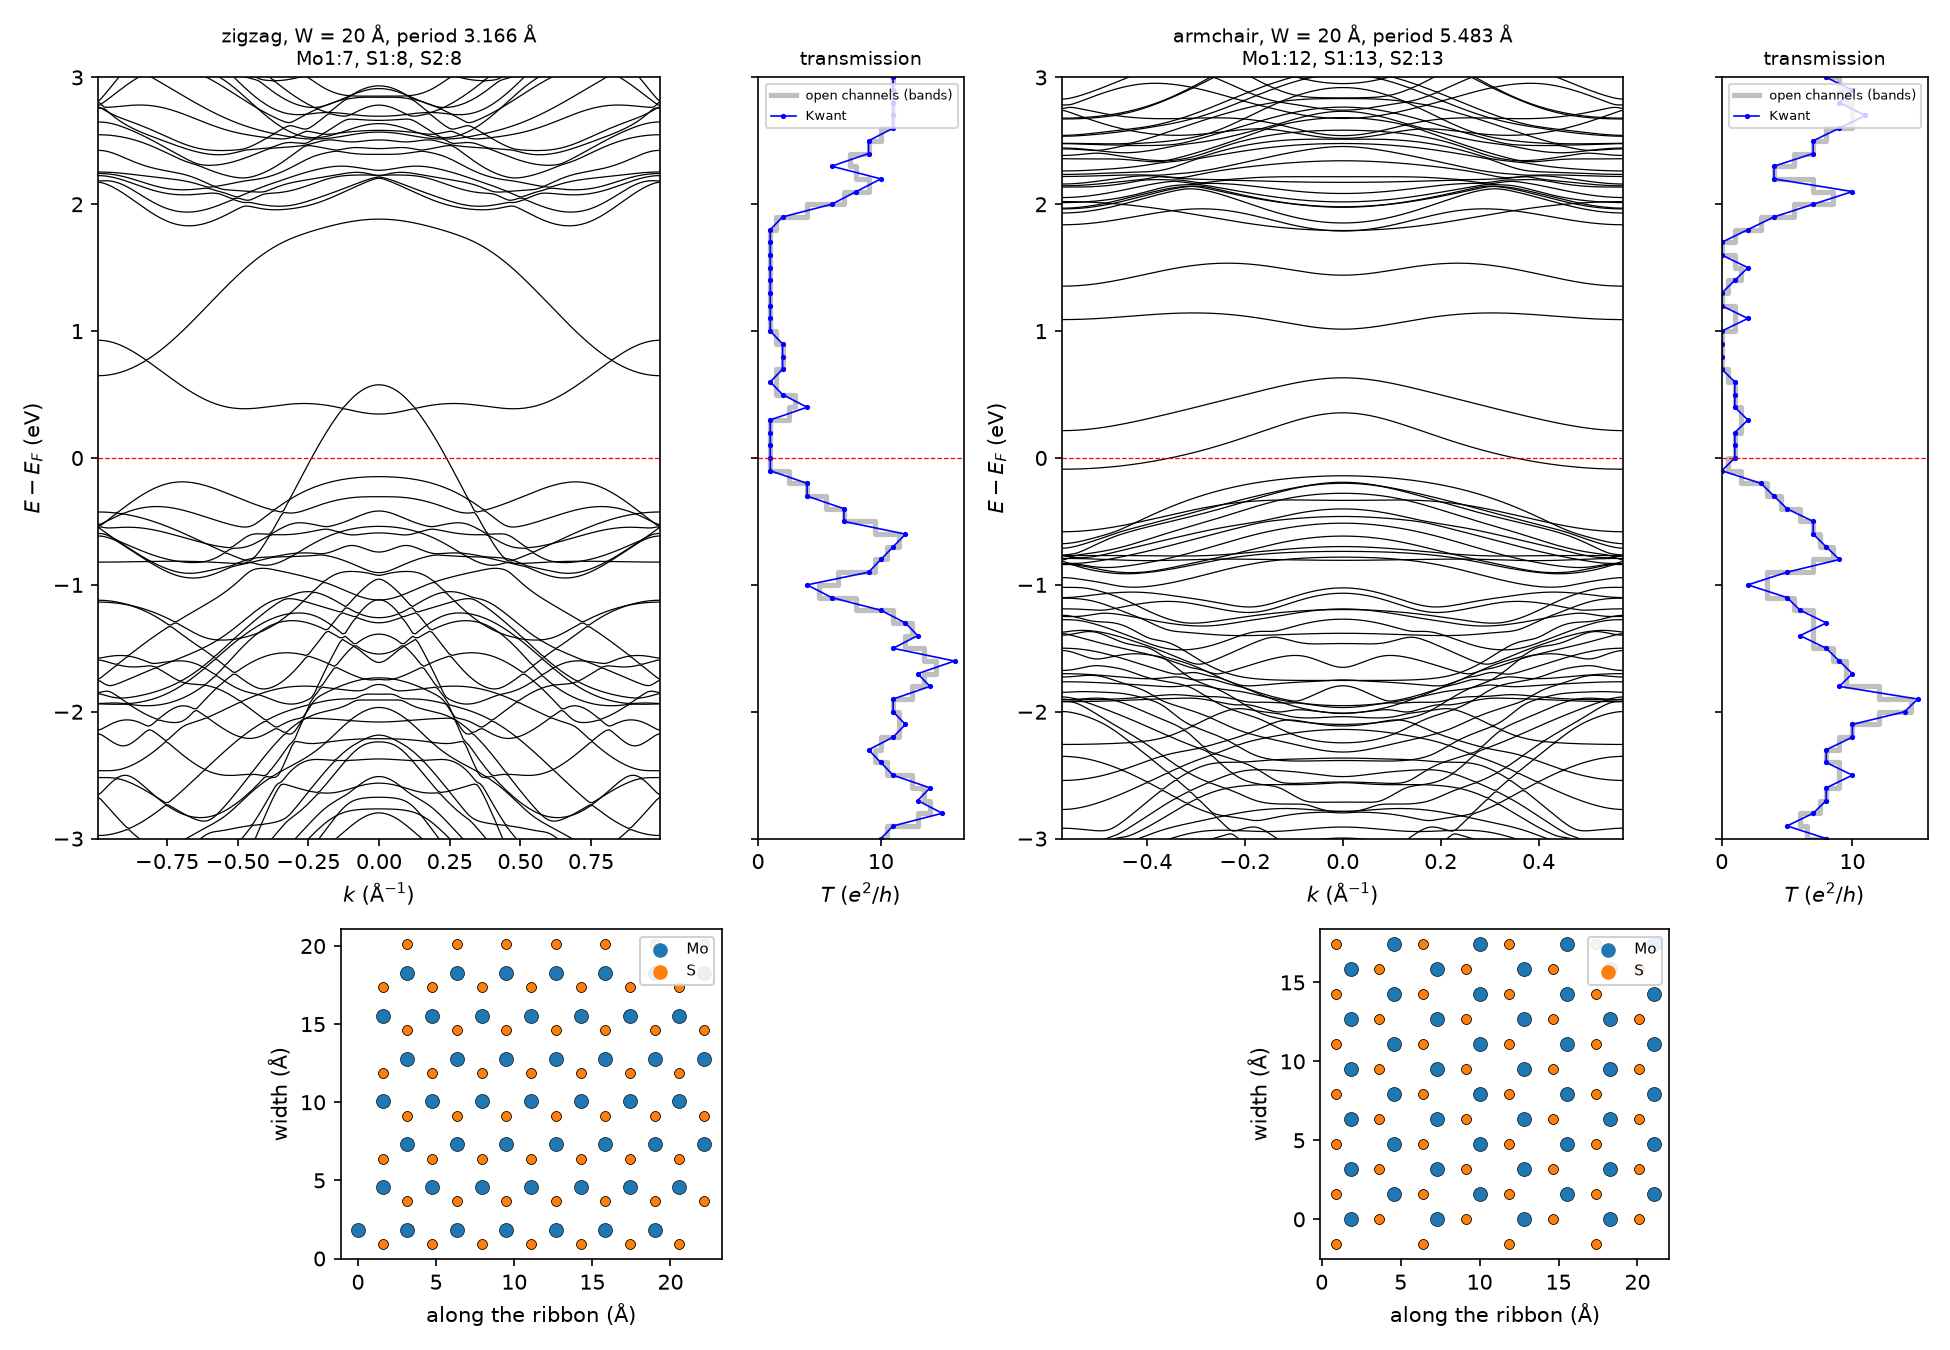
\includegraphics[width=\linewidth]{figures/bands_ribbons.png}
\caption{MoS$_2$ nanoribbons, $W=20$\,\AA, produced by \code{python kwant\_model.py}.
Top: band structures and Kwant transmission (blue), compared with the number of open
channels counted from the bands (grey). Bottom: top views of the ribbons.}
\label{fig:ribbons}
\end{figure}

\subsection{Current--voltage characteristics}\label{sec:iv}
The current is obtained from the Landauer formula,
\begin{equation}
  I(V) = g_s\,\frac{e}{h}\int T(E)\,\big[f(E-\mu_L) - f(E-\mu_R)\big]\,dE,
  \qquad \mu_{L,R} = E_F \pm \frac{eV}{2},
\end{equation}
where $f$ is the Fermi--Dirac distribution, and $g_s=2$ for spin-degenerate (NP) models
and $g_s=1$ for SP/SOC models, whose $T$ already includes both spins.
With $T$ in units of $e^2/h$ and energies in eV, $I[\mu\text{A}] = 38.74\,g_s\int T\,(f_L-f_R)\,dE$.
Two approximations are made:
\begin{itemize}[nosep]
  \item \textbf{Rigid band:} $T(E)$ is computed at zero bias. There is no potential drop
        or self-consistent charge redistribution in the scattering region; only the
        Fermi windows of the leads move.
  \item \textbf{Cheaper Hamiltonian:} to make the fine energy grid affordable, hoppings with
        $|H|<10^{-3}$\,eV are dropped. As shown in the bulk table above, this changes the
        bands by up to 31\,meV. It also reduces the lead supercells from $N=9$ to $N=5$
        (zigzag) and from $N=4$ to $N=3$ (armchair).
\end{itemize}
The implementation was checked against the analytic case $T=1$, which gives
$I/V = 2e^2/h = 77.48\,\mu$A/V for $g_s=2$.

Figure~\ref{fig:iv} shows $T(E)$ (355 energies, step 0.01\,eV) and the $I$--$V$ curves
from 0 to 3\,V at 300\,K for the 20\,\AA{} MoS$_2$ ribbons, obtained with
\code{python kwant\_model.py --iv}. With 12 processes the whole calculation took
2.7\,minutes: 51\,s for the zigzag ribbon and 108\,s for the armchair ribbon. Selected
values are listed in Table~\ref{tab:iv}.

\begin{itemize}[nosep]
  \item \textbf{Low bias:} both ribbons have a single channel at $E_F$, so
        $dI/dV|_{V\to0}\approx 2e^2/h$ ($77.9$ and $74.6\,\mu$A/V for zigzag and
        armchair).
  \item \textbf{Above about 0.4\,V:} the bias window starts to include the valence
        band. The current then rises steeply, much more in the zigzag ribbon, which has
        more channels below $E_F$.
  \item \textbf{Plateau around 2\,V:} it reflects the reduced number of channels between
        about 1 and 1.8\,eV above $E_F$.
\end{itemize}
These curves are rigid-band estimates for perfect ribbons. They are meant as a
demonstration of the workflow, not as a quantitative prediction of device
characteristics.

\begin{table}[h]
\centering
\caption{Landauer current of 20\,\AA{} MoS$_2$ ribbons (300\,K, hopping cutoff $10^{-3}$\,eV).}
\label{tab:iv}
\begin{tabular}{lcccccc}
\toprule
$V$ (V)            & 0.5  & 1.0   & 1.5   & 2.0   & 2.5   & 3.0 \\
\midrule
$I_\text{zigzag}$ ($\mu$A)   & 57.2 & 207.8 & 409.1 & 574.1 & 745.7 & 994.3 \\
$I_\text{armchair}$ ($\mu$A) & 47.6 & 173.3 & 330.5 & 422.8 & 531.3 & 681.7 \\
\bottomrule
\end{tabular}
\end{table}

\begin{figure}[h]
\centering
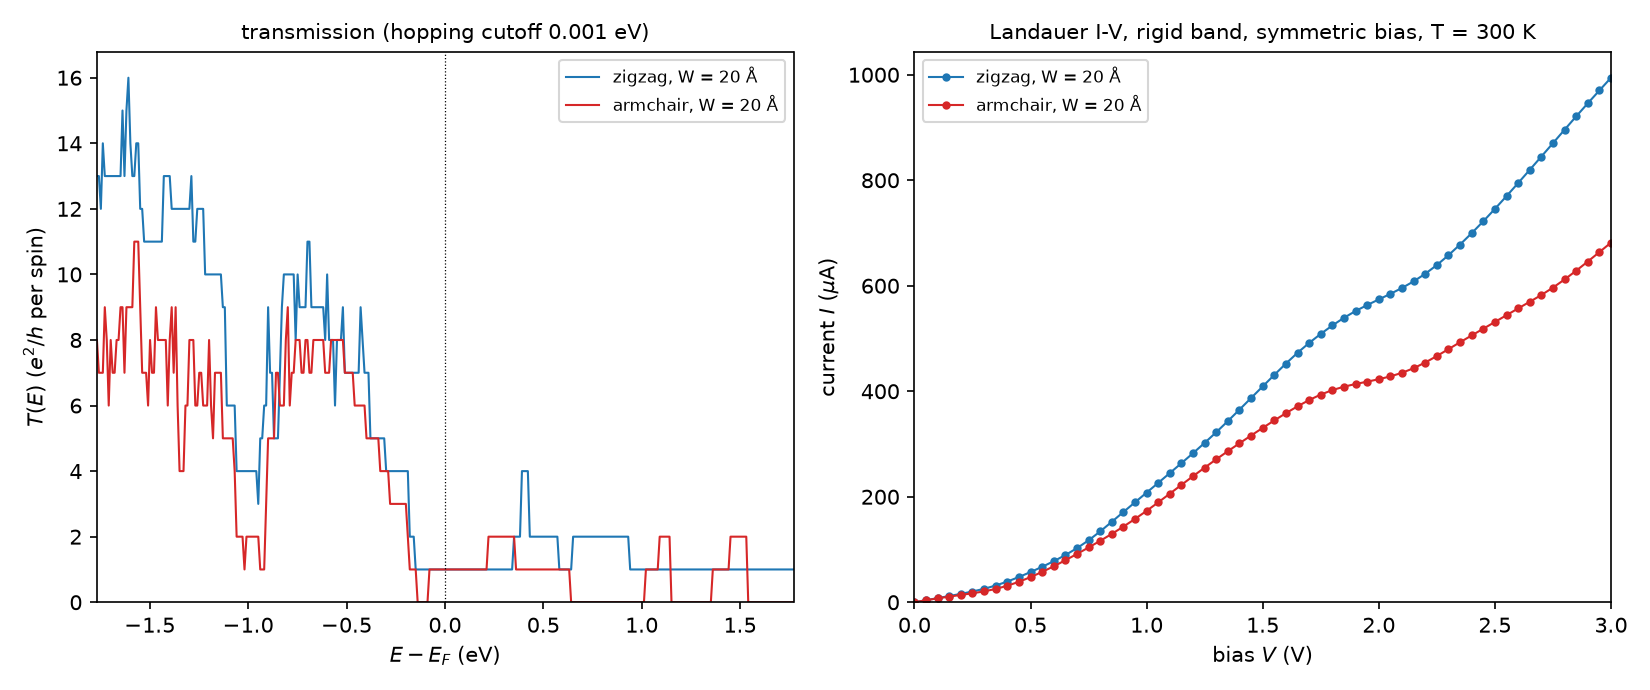
\includegraphics[width=\linewidth]{figures/iv_ribbons.png}
\caption{Left: transmission of the 20\,\AA{} zigzag and armchair MoS$_2$ ribbons computed
with the cheaper Hamiltonian (hopping cutoff $10^{-3}$\,eV). Right: Landauer $I$--$V$
curves in the rigid-band approximation, with symmetric bias and $T=300$\,K.}
\label{fig:iv}
\end{figure}

\paragraph{Effect of the cheaper Hamiltonian.}
At the 35 energies in $[-1.7, 1.7]$\,eV shared with the full-model calculation of
Figure~\ref{fig:ribbons}, the transmission of the cut Hamiltonian is identical in 33/35
(zigzag) and 32/35 (armchair) points. The differences, of at most 2 channels, occur next
to band edges, which the 31\,meV band shifts move across the sampled energy. The $I$--$V$
curves are therefore reliable on the scale of the figure. For quantitative work, repeat the
calculation with \code{--hop-cutoff 0}.

\subsection{Running the tests}
\begin{lstlisting}[language=bash]
python -m pytest tests -q            # fast regression tests
python tests/validate_mos2_np.py     # full report (several minutes)
\end{lstlisting}
Both scripts use the MoS$_2$ data set that ships with the repository in
\code{tests/data/mos2\_np/} (\code{tb\_hr.dat}, \code{wannier90.wout}, \code{wannier90.win}
and the Wannier90 band-structure files). To use another data set, set the environment
variable \code{WTB2KWANT\_MOS2\_DIR}. The validation script accepts \code{--quick} (no
transmission in the example and no $I$--$V$, about 5\,min) and \code{--skip-iv}. The full
run takes about 13\,min on 12 cores.

%=====================================================================
\section{Limitations and roadmap}\label{sec:roadmap}
%=====================================================================
\begin{itemize}
  \item \textbf{$I$--$V$ beyond the rigid-band picture:} include a bias-dependent
        electrostatic potential (for example a linear drop or a self-consistent
        Poisson solution) as on-site terms that depend on Kwant \code{params}.
  \item \textbf{Non-orthogonal Hamiltonians (SIESTA, \code{tb-*.ham}).} Kwant has no
        overlap matrix. At a fixed energy $E$, the generalized problem
        $(H-ES)\psi=0$ is equivalent to $(H'-E)\psi=0$ with
        \begin{equation}
          H' = H - E\,(S - \mathbb{1}).
        \end{equation}
        The plan is to make the on-site terms and hoppings functions of $E$ passed through
        \code{params}. This gives exact transmissions. Bands and DOS require solving the
        generalized eigenproblem directly.
  \item \textbf{Nanotubes:} roll the 2D sheet along a chiral vector $\mathbf{C}_h=(n,m)$
        with periodic boundary conditions, neglecting curvature corrections to the
        hoppings.
  \item \textbf{3D crystals and slabs:} at present only systems with two periodic
        directions are supported.
  \item \textbf{SP and SOC:} implemented but not yet validated with reference data.
  \item \textbf{Scissors operator:} not applied.
\end{itemize}

%=====================================================================
\appendix
\section{Repository layout}
%=====================================================================
\begin{lstlisting}
wtb2kwant/
  wtb2kwant/readers.py    readers: tb_hr.dat, wannier90.wout
  wtb2kwant/model.py      TBModel, site assignment, folding, cutoff
  wtb2kwant/codegen.py    generator of the Kwant script
  wtb2kwant/cli.py        command-line interface
  tests/                  pytest tests, validation script and results
  tests/data/mos2_np/     MoS2 test data (Wannier90/VASP)
  bin/                    launchers written by install.sh (not versioned)
  manual/                 this manual (LaTeX)
  install.sh              conda installer
  pyproject.toml, README.md, LICENSE (MIT)
\end{lstlisting}

\section{License}
\tool{} is distributed under the MIT License (see the file \code{LICENSE} in the repository).

\end{document}
